\documentclass{article}
\usepackage[utf8]{inputenc}
\usepackage{graphicx}
\usepackage{multicol}
\usepackage{caption}
\usepackage{makecell}
\usepackage{algpseudocode}  % sudo apt-get install texlive-science
\usepackage{algorithm}
\usepackage[hidelinks]{hyperref}
\hypersetup{
    colorlinks=true,
    linkcolor=blue,     
    urlcolor=blue,
    }
\usepackage{verbatim}


\vspace{\stretch{1}}

\title{\LARGE Parallel Mean Shift Clustering \\
\large Elaborato Parallel Programming For Machine Learning}
\author{Nicol\'o Pollini, Francesco Fantechi}
\date{A.A. 2022-2023}

\begin{document}

\maketitle

\begin{figure}[!h]
\centering

\includegraphics[width=4cm, height=4cm]{"Immagini/LogoUnifi.PNG"}
\end{figure}

\begin{center}
\textbf{\large UNIVERSITA' DEGLI STUDI DI FIRENZE \\
Facolta di Ingegneria \\
\normalsize Corso di Laurea Magistrale in Ingegneria Informatica}
\end{center}

\vspace{\stretch{1}}

\newpage

% Indice
\tableofcontents

\newpage

\section{Obiettivo}

L'obiettivo di questo progetto è quello di parallelizzare l'algoritmo di clustering Mean Shift tramite il framework OpenMP e l'architettura hardware CUDA e mettere a confronto i due metodi valutando gli speedup ottenuti rispetto all'esecuzione sequenziale.  

\section{Mean Shift}
Mean Shift è un algoritmo che permette di clusterizzare un insieme $ N $ di punti appartenenti ad uno spazio delle feature a $ n $ dimensioni con un metodo equivalente all'applicazione della discesa del gradiente. L'algoritmo clusterizza i punti assegnadoli alla propria $ mode $, ossia il punto a massima densit\'a nello spazio delle feature che gli influenza di pi\'u. Per ogni punto viene infatti inizializzata la propria media con il proprio valore. Viene successivamente calcolato il centroide dei punti contenuti in una sfera di raggio $bandwidth$ centrata nella media corrente. Questo valore appena calcolato viene poi assegnato alla media del punto e si procede ripetendo questo procedimento fino a che lo scostamento fra i due non risulti inferiore ad una certa soglia $\varepsilon$. Spostare la media nel centroide equivale a compiere un passo dell'algoritmo di discesa del gradiente applicato alla funzione densit\'a (Vedi Figura \ref{2D_Mean_Shift_simualtion_view}). Raggiunto il termine del procediemnto, la media conterr\'a la $mode$ del punto cercata alla quale quet'ultimo verr\'a assegnato. Questo algoritmo risulta computazionalmente complesso $(\mathcal{O}(n^{2}))$ ma presenta i vantaggi di essere semplice, di non necessitare di inizializzazione, di trovare un numero di cluster arbitrario e non definito a priori e di essere robusto agli outliers. Il numero di clustering trovati e la loro dimensione dipendono dal parametro $bandwidth$ scelto.    

\begin{figure}[!h]
\centering
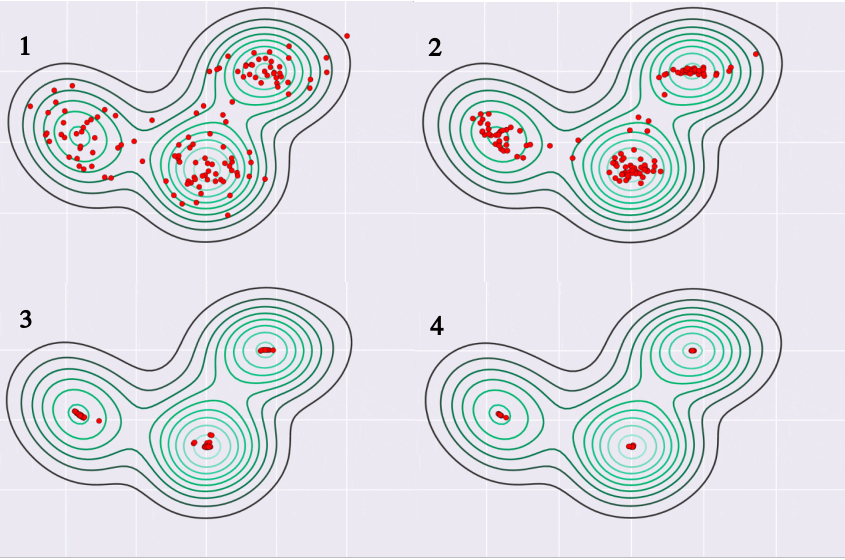
\includegraphics[width= 9.5cm]{"Immagini/Simulation.PNG"}
\caption{2D Mean Shift simulation view}
\label{2D_Mean_Shift_simualtion_view}
\end{figure}

\newpage


\subsection{Pseudocodice} \label{Pseudocodice}
\begin{algorithm}
\caption{Mean Shift algorithm}\label{euclid}
\begin{algorithmic}[1]
\Procedure{MeanShift}{$N$}\Comment{The clustering of $ N $ points in feature space}
\State $shift\gets\varepsilon $
\State $M\gets[$ $] $
\ForAll{$ i $ in $ N $}
\State $ m_{i} \gets i $\Comment{Initial mean for each point}
\While{$shift\geq\varepsilon$}\Comment{Stop if $shift$ less than a threshold $ \varepsilon $}
\State $sum=0$
\For{$ j \in N $ in $ Ball_{bandwidth}(m_{i})$}
\State $sum\gets j$
\EndFor
\State $centroid\gets sum/|Ball_{bandwidth}(m_{i})|$
\State $shift \gets distance(m_{i},centroid)$
\State $m_{i} \gets centroid$
\EndWhile\label{euclidendwhile}
\State $M \gets M\cup m_{i}$\Comment{$M$ contains the modes of the points}
\EndFor
\State \textbf{return} $M$
\EndProcedure
\end{algorithmic}
\end{algorithm}

\section{Procedimento e implementazione}

L'algoritmo Mean Shift \'e stato valutato e confrontato nella clusterizzaione di immagini in formato “.ppm” di differenti dimensioni. I nostri punti da clusterizzare saranno quindi tanti quanti i pixel che compongono l'immagine e saranno dei valori appartenenti ad uno spazio $5$-dimensionale: il valore dei tre canali colore Rosso, Verde e Blu, e la posizione lungo l'asse delle ascisse e delle ordinate del pixel nell'immagine.\\
\\
\noindent L'intero progetto è stato implementato in linguaggio C++ ed \'e stato eseguito su tre diverse macchine le cui caratteristiche sono riportate in Tabella \ref{Technical Specifications}. Il codice \'e stato versionato tramite la piattaforma GitHub ed \'e reperibile ai siti:\\
\url{https://github.com/francesco-ftk/Parallel-Mean-Shift-OpenMP.git} \\
\url{https://github.com/francesco-ftk/Parallel-Mean-Shift-CUDA.git}\\
\\
\noindent Il progetto pu\'o essere suddiviso in tre parti:
\begin{enumerate}
\item Implemenatazione dell'agoritmo Mean Shift in modo sequenziale
\item Parallelizzazione dell'algoritmo Mean Shift tramite il framework OpenMP
\item Parallelizzazione dell'algoritmo Mean Shift tramite l'architettura CUDA
\end{enumerate}

\newpage

\subsection{Mean Shift Sequenziale}

Sono state implementati due diversi modelli di design dell'algoritmo Mean Shift a seconda del layout dei dati utilizzato.\\ La prima versione utilizza una struttura dati a matrice per la gestione dei punti da clusterizzare. Questa tipo di struttura denominata “Array of Structures” (AoS) prevede infatti che i nostri punti $5$-dimensionali siano collocati sequenzialmente in un unico vettore. Tenendo i dati localmente vicini, la struttura AoS risulta vantaggiosa per poter accedere agli elementi nel loro complesso.\\ La seconda versione utilizza invece una struttura dati denominata “Structure of Arrays” (SoA). Questa struttura prevede che i nostri punti $5$-dimensionali siano divisi in cinque array ognuno contenente uno specifio tipo di dato. La struttura SoA per la sua forma risulta pi\'u facilmente allineabile con la memoria cache ma necessita di un numero maggiore di accessi alla memoria per riunire i dati (Vedi Figura \ref{Data Layout}).\\
\\
Entrambe le versioni sono state eseguite sull'ambiente di sviluppo CLion in modalit\'a “Debug” di modo da non introddure parallelizzazioni implicite da parte dell'IDE. I tempi di esecuzione in millisecondi presi su una media di dieci esecuzioni sono riportati in Tabella \ref{Timings}. In figura \ref{Output} \'e possibile visualizzare l'output ottenuto dall'algoritmo.

\vspace{10px}    

\begin{figure}[!h]
\centering
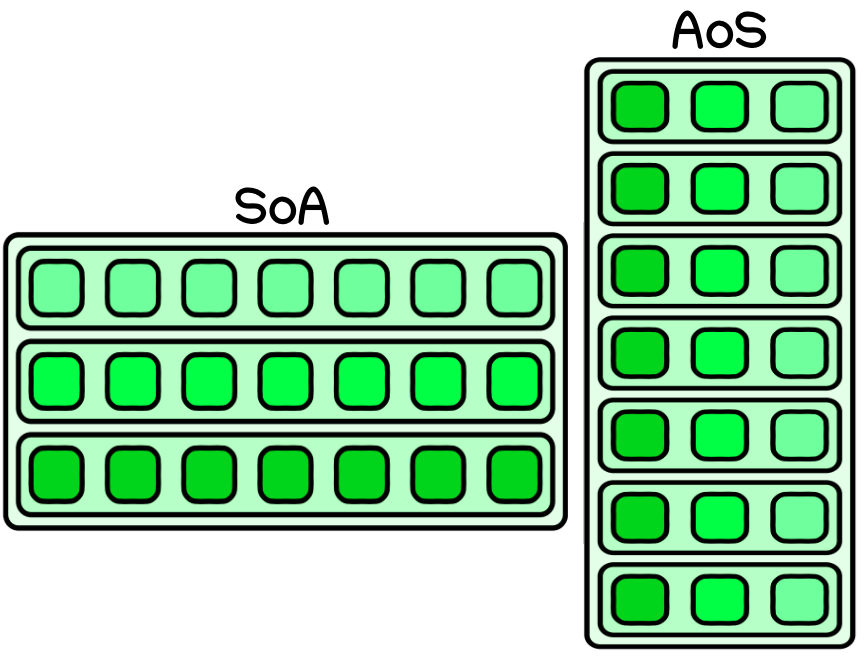
\includegraphics[width= 10cm]{"Immagini/Data_Layout.PNG"}
\caption{Data Layout: Soa vs. Aos}
\label{Data Layout}
\end{figure}

\newpage


\subsection{OpenMP}
OpenMP \'e un framework che permette di parallelizzare una porzione di codice in modalit\'a implicit threading attraverso delle direttive “pragma”.\\
Il nostro algoritmo sequenziale pu\'o essere diviso in due parti: la prima nella quale viene calcolata per ogni punto la propria mode attraverso l'algoritmo sopra riportato (vedi \ref{Pseudocodice}), e la seconda nella quale i punti vengono effettivamente clusterizzati assieme a seconda della vicinanza fra le loro mode. Nella prima parte i punti calcolano la loro mode in modo indipendente l'uno dagli altri. Questa sezione risuta quindi imbarazzantemente parallela e quindi facilmente parallelizzabile in quanto i thread non necessitano di comunicare o scambiare informazioni fra di loro (vedi Figura \ref{Code OpenMP}). La secoda parte non essendo imbarazzantemente parallela non \'e stata parallelizzata invece.\\
\\
Il numero di thread usati da ogni macchina \'e stato calcolato aggiungendo un $ 50\% $ al numero complessivo di Core posseduti considerando l'Hyper-Threading (vedi Tabella \ref{Technical Specifications}).
I tempi di completamento in millisecondi presi su una media di dieci esecuzioni in modialit\'a “Debug” sono riportati in Tabella \ref{Timings}. Con questi tempi $ t^{p} $ e quelli presi tramite l'implementazione sequenziale $ t^{s} $ sono stati successivamente calcolati gli speedup delle due versioni tramite la formula $ S=t^{s}/t^{p} $. Questi ultimi sono osservabili in Tabella \ref{Speedups}.

\vspace{10px}

\begin{figure}[!h]
\centering
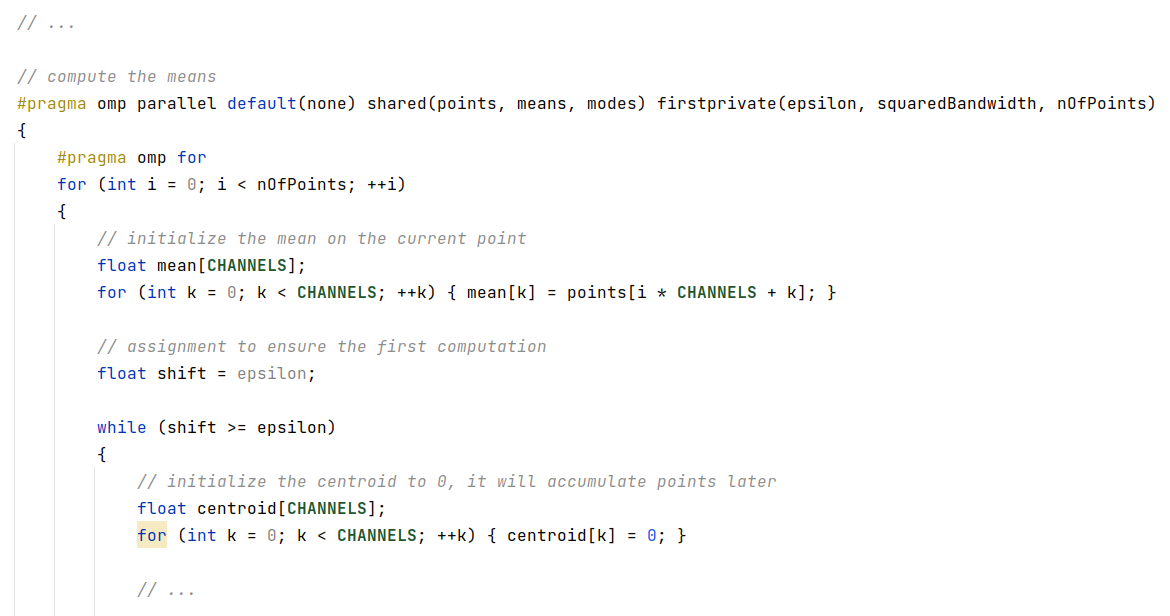
\includegraphics[width= 15cm]{"Immagini/Code_OpenMP.PNG"}
\caption{Piece of code parallelized via OpenMP}
\label{Code OpenMP}
\end{figure}

\newpage

\subsection{CUDA}

CUDA \'e un'architettura hardware che permette di parallelizzare dei programmi general purpose eseguendo parallelamnete molti thread sulle GPU NVIDIA. La GPU (device) \'e vista come coprocessore della CPU (host) ed \'e possibile gestirne completamente la memoria. Le architetture Nvidia possiedono molteplici strutture di memoria ognuna delle quali \'e caratterizzata da una diversa capacit\'a, velocit\'a di accesso e condivisibilit\'a dei dati. Infatti, come mostrato in figura \ref{Memory}, queste dispongono non solo di una memoria principale (Global Memory) e di una memoria costante (Constant Memory, non modificabile dai programmi device) a cui tutti i thread possono accedere, ma anche di una memoria condivisa a livello di blocco, chiamata Shared Memory. La velocit\'a di accesso alla Shared Memory \'e significativamente pi\'u alta rispetto alla Global Memory, tuttavia una sua limitazione \'e la dimensione. Non potendo contenere tutti i dati di input contemporaneamente, dopo aver portato i punti da clusterizzare da host a device, per velocizzare il loro accesso da parte dei thread dei blocchi, questi sono stati portati al momento del bisogno dalla Global Memory alla Shared Memory dei vari blocchi tramite una strategia di Tiling.

\vspace{30px}

\begin{figure}[!h]
\centering
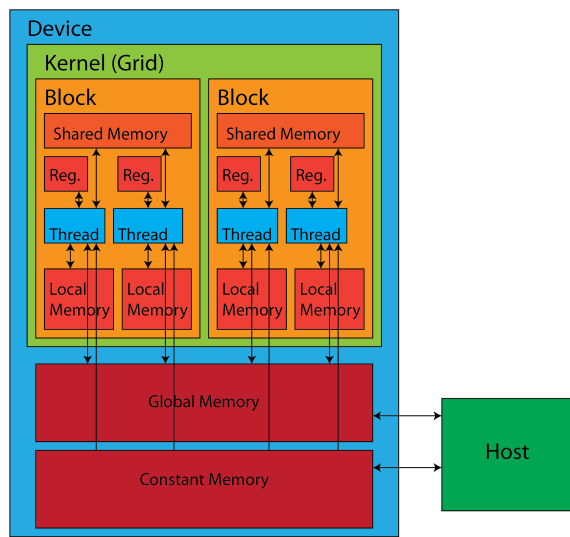
\includegraphics[width= 9cm]{"Immagini/Memory.PNG"}
\caption{GPU memory view}
\label{Memory}
\end{figure} 

\newpage

\noindent Il Tiling, come si pu\'o osservare in figura \ref{tilings-loops} e \ref{tiling}, consiste nel dividere lo spazio dei dati in pi\'u parti e sottoporre ogni blocco di thread ad una esecuzione in pi\'u fasi durante ognuna delle quali una sola parte dei dati viene utilizzata per la computazione. Durante le varie fasi, ogni thread è responsabile del caricamento in Shared Memory di una porzione di dati che sarà potenzialmente utilizzata da tutti i thread appartenenti allo stesso blocco, perci\'o \'e cruciale che questa operazione venga eseguita tramite delle barriere di sincronizzazione.

\vspace{15px}

\begin{figure}[!h]
\centering
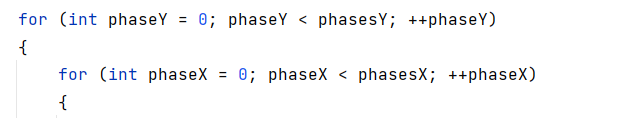
\includegraphics[width= 10cm]{"Immagini/tiling-loops.PNG"}
\caption{Multi-phase execution due to Tiling}
\label{tilings-loops}
\end{figure}

\vspace{15px}

\begin{figure}[!h]
\centering
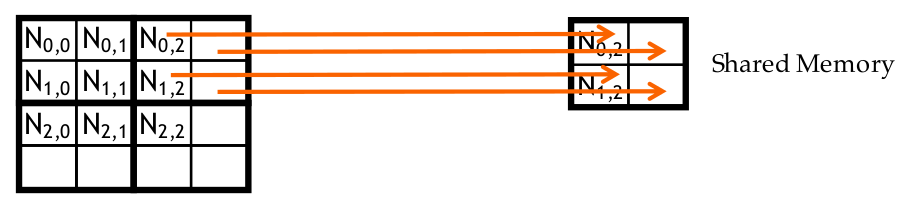
\includegraphics[width= 10cm]{"Immagini/Tiling.PNG"}
\caption{PhaseY$=0 $ PhaseX$=1 $ Tiling simulation}
\label{tiling}
\end{figure}

\vspace{15px}

\noindent Nel caso del Kernel sviluppato per l'algoritmo Mean Shift, ogni thread ha la responsabilit\'a di calcolare la mode di un singolo pixel. Per farlo deve completare un numero indefinito di iterazioni  su tutte le fasi, all'interno delle quali il pixel viene sottoposto ad una serie di operazioni che utilizzano, uno ad uno, ogni altro pixel dell'immagine. Poich\'e i dati di input vengono quindi utilizzati da più thread, questi sono stati portati sulla shared memory e condivisi a livello di blocco. Durante ogni iterazione, ogni blocco di thread carica in modo sincronizzato una porzione di dati in Shared Memory (vedi figura \ref{shared-load}), la consuma (vedi figura \ref{shared-consume}), e ripete queste due operazioni per un numero di fasi sufficiente a terminare i dati complessivi.

\newpage

\vspace{30px}

\begin{figure}[!h]
\centering
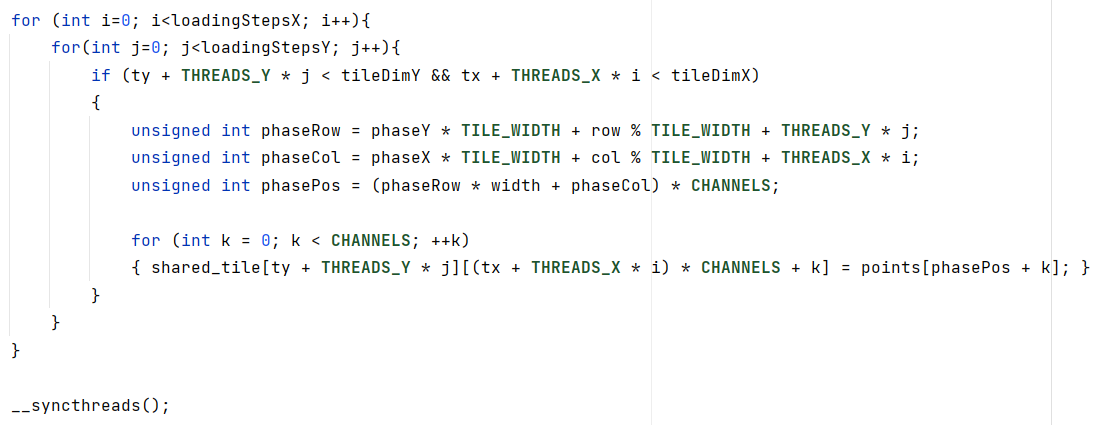
\includegraphics[width= 12cm]{"Immagini/shared-load.PNG"}
\caption{Loading in Shared Memory of the portion of data corresponding to the current phase}
\label{shared-load}
\end{figure}

\vspace{30px}

\begin{figure}[!h]
\centering
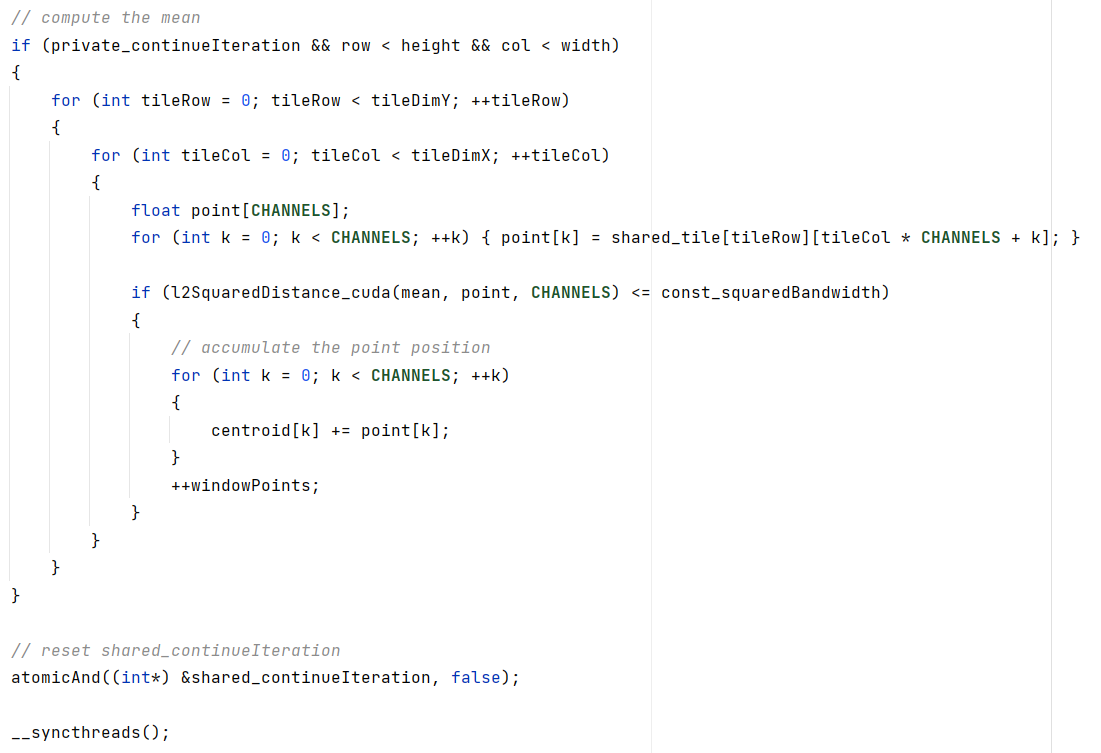
\includegraphics[width= 12cm]{"Immagini/shared-consume.PNG"}
\caption{Consumption of the loaded portion of data}
\label{shared-consume}
\end{figure}

\newpage 

\vspace{30px}

\noindent Tuttavia, per costruzione dell'algoritmo, il numero di iterazioni che ogni thread deve eseguire per calcolare la mode del proprio pixel \'e variabile e non prevedibile. In altre parole, alcuni thread potrebbero necessitare di meno iterazioni di altri, e ci\'o risulterebbe incompatibile con il caricamento sincronizzato dei dati in Shared Memory. Per gestire questo problema sono state utilizzate due variabili booleane di cui una condivisa a livello di blocco. La variabile condivisa (vedi figura \ref{shared-variable}) ha lo scopo di informare l'intero blocco di thread della necessit\'a di continuare con una nuova iterazione, a causa della presenza di almeno uno di loro che non ha terminato la propria esecuzione. La variabile privata invece (vedi figura \ref{shared-consume} e \ref{iteration-end}) tiene traccia della necessit\'a effettiva per un thread di consumare i dati, oltre che caricarli.\\ Una volta che tutti i thread hanno terminato le loro iterazioni il kernel pu\'o finalmente terminare. I dati delle mode dei pixel vengono copiati indietro sulla memoria host e l'esecuzione sequenziale per il conteggio dei cluster viene avviata.

\vspace{30px}

\begin{figure}[!h]
\centering
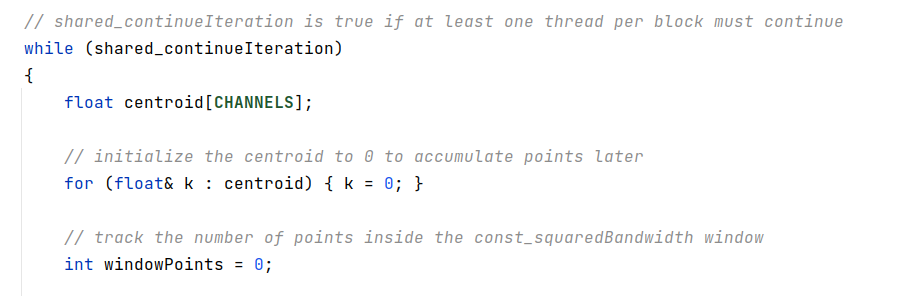
\includegraphics[width= 11cm]{"Immagini/shared-variable.PNG"}
\caption{Start of a new iteration if at least one thread has not completed the mode calculation}
\label{shared-variable}
\end{figure}

\newpage

\vspace{30px}

\begin{figure}[!h]
\centering
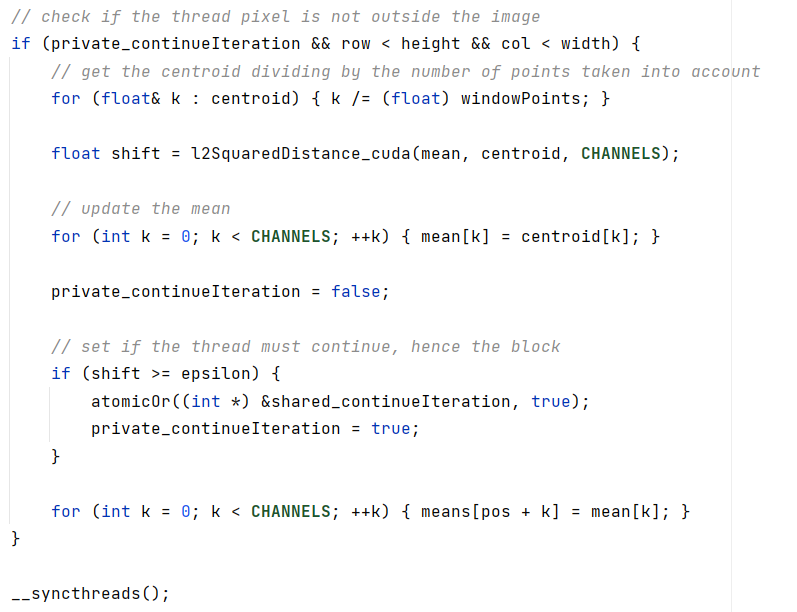
\includegraphics[width= 11cm]{"Immagini/iteration-end.PNG"}
\caption{Check if mode computation is finished or another iteration is to be done}
\label{iteration-end}
\end{figure}

\vspace{30px}

\noindent Solo la versione sequenziale AoS di Mean Shift \'e stata parallelizzata tramite CUDA e il suo tempo di completamento in millisecondi preso su una media di dieci esecuzioni con un tile di $ 8\times8 $ pixel \'e riportato in Tabella \ref{Timings}. In Tabella \ref{Speedups} \'e possibile osservare lo speedup successivamente calcolato rispetto all'esecuzione sequenziale AoS. In figura \ref{Speedups_Varying_Size} \'e riportato inoltre un grafico che mostra l'andamento dello speedup ottenuto dalla macchina $ 3 $ (vedi Tabella \ref{Technical Specifications}) al variare della dimensione dell'immagine da clusterizzare utilizzando un tiling $ 8\times8 $ e $ 16\times16 $, mentre in figura \ref{Timings_Varying_Tile} \'e riporato invece un grafico che mostra i tempi di esecuzione della macchina $ 3 $ (vedi Tabella \ref{Technical Specifications}) al variare della dimensione del tiling su un'immagine di dimensione $ 100\times100 $ pixel.   

\newpage

\section{Risultati}

\begin{figure}[!h]
\centering
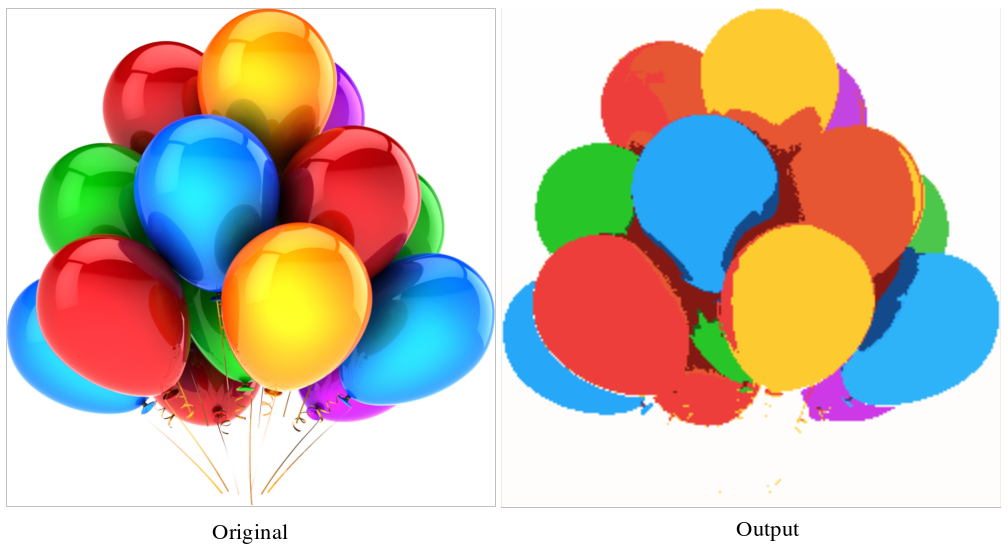
\includegraphics[width= 13cm]{"Immagini/Output.PNG"}
\caption{Mean Shift Algorithm Output}
\label{Output}
\end{figure}

\begin{center}
\captionof{table}{Machine's technical specifications} \label{Technical Specifications}
\begin{tabular}{|c|c|c|c|c|}
\hline
\multicolumn{5}{|c|}{Machine 1}\\
\hline
\thead{OS} & \thead{CPU} & \thead{Number of Core \\ with Hyper-Threading} & \thead{RAM} & \thead{GPU}\\
\hline
\thead{Windows $ 10 $} & \thead{Intel(R) Core(TM) \\ i7-8750H} & \thead{$ 12 $} & \thead{$ 16 $ GB} & \thead{NVIDIA GeForce \\ GTX 1050 Ti}\\
\hline
\multicolumn{5}{|c|}{}\\
\hline
\multicolumn{5}{|c|}{Machine 2}\\
\hline
\thead{OS} & \thead{CPU} & \thead{Number of Core \\ with Hyper-Threading} & \thead{RAM} & \thead{GPU}\\
\hline
\thead{Ubuntu $ 20.04.5 $} & \thead{Intel(R) Core(TM) \\ i7-1165G7} & \thead{$ 8 $} & \thead{$ 16 $ GB} & \thead{NVIDIA GeForce \\ MX350}\\
\hline
\multicolumn{5}{|c|}{}\\
\hline
\multicolumn{5}{|c|}{Machine 3}\\
\hline
\thead{OS} & \thead{CPU} & \thead{Number of Core \\ with Hyper-Threading} & \thead{RAM} & \thead{GPU}\\
\hline
\thead{Windows $ 10 $} & \thead{Intel(R) Core(TM) \\ i7-7700K} & \thead{$ 8 $} & \thead{$ 32 $ GB} & \thead{NVIDIA GeForce \\ GTX 1080 Ti}\\
\hline
\end{tabular}

\captionof{table}{Timings} \label{Timings}
\begin{tabular}{|c|c|c|c|c|c|}
\hline
\multicolumn{6}{|c|}{Machine 1}\\
\hline
\thead{Image dimension} & \thead{Sequential AoS} & \thead{Sequential SoA} & \thead{OpenMP AoS} & \thead{OpenMP SoA} & \thead{CUDA}\\
\hline
\thead{$ 100\times100$ pixel} & \thead{$ 102810ms$} & \thead{$ 102188ms $} & \thead{$  17047ms $}  & \thead{$  15657ms $} & \thead{$  10477ms $}\\
\hline
\thead{$ 250\times250$ pixel} & \thead{$ 3955082ms $} & \thead{$ 3886222ms $} & \thead{$ 575754ms $}  & \thead{$ 554569ms $} & \thead{$ 276233ms $}\\
\hline
\multicolumn{6}{|c|}{}\\
\hline
\multicolumn{6}{|c|}{Machine 2}\\
\hline
\thead{Image dimension} & \thead{Sequential AoS} & \thead{Sequential SoA} & \thead{OpenMP AoS} & \thead{OpenMP SoA} & \thead{CUDA}\\
\hline
\thead{$ 100\times100$ pixel} & \thead{$ 37370ms $} & \thead{$ 35758ms $} & \thead{$ 9937ms $}  & \thead{$ 10056ms $} & \thead{$ 12892ms $}\\
\hline
\thead{$ 250\times250$ pixel} & \thead{$ 1442048ms $} & \thead{$ 1393829ms $} & \thead{$ 467553ms $}  & \thead{$ 494691ms $} & \thead{$ 355589ms $}\\
\hline
\multicolumn{6}{|c|}{}\\
\hline
\multicolumn{6}{|c|}{Machine 3}\\
\hline
\thead{Image dimension} & \thead{Sequential AoS} & \thead{Sequential SoA} & \thead{OpenMP AoS} & \thead{OpenMP SoA} & \thead{CUDA}\\
\hline
\thead{$ 100\times100$ pixel} & \thead{$ 87317ms $} & \thead{$ 86241ms $} & \thead{$ 16547ms $}  & \thead{$ 15367ms $} & \thead{$ 3009ms $}\\
\hline
\thead{$ 250\times250$ pixel} & \thead{$ 3339803ms $} & \thead{$ 3309131ms $} & \thead{$ 601750ms $}  & \thead{$ 574439ms $} & \thead{$ 56213ms  $}\\
\hline
\end{tabular}

\vspace{30px}

\captionof{table}{Speedups} \label{Speedups}
\begin{tabular}{|c|c|c|c|}
\hline
\multicolumn{4}{|c|}{Machine 1}\\
\hline
\thead{Image dimension} & \thead{OpenMP AoS} & \thead{OpenMP SoA} & \thead{CUDA}\\
\hline
\thead{$ 100\times100$ pixel} & \thead{$ 6.0 $}  & \thead{$ 6.5 $} & \thead{$ 9.8 $}\\
\hline
\thead{$ 250\times250$ pixel} & \thead{$ 6.9 $}  & \thead{$ 7.0 $} & \thead{$ 14 $}\\
\hline
\multicolumn{4}{|c|}{}\\
\hline
\multicolumn{4}{|c|}{Machine 2}\\
\hline
\thead{Image dimension} & \thead{OpenMP AoS} & \thead{OpenMP SoA} & \thead{CUDA}\\
\hline
\thead{$ 100\times100$ pixel} & \thead{$ 3.7 $}  & \thead{$ 3.6 $} & \thead{$ 2.9 $}\\
\hline
\thead{$ 250\times250$ pixel} & \thead{$ 3.0 $}  & \thead{$ 2.8 $} & \thead{$ 4.1 $}\\
\hline
\multicolumn{4}{|c|}{}\\
\hline
\multicolumn{4}{|c|}{Machine 3}\\
\hline
\thead{Image dimension} & \thead{OpenMP AoS} & \thead{OpenMP SoA} & \thead{CUDA}\\
\hline
\thead{$ 100\times100$ pixel} & \thead{$ 5.3 $}  & \thead{$ 5.6 $} & \thead{$ 29.0 $}\\
\hline
\thead{$ 250\times250$ pixel} & \thead{$ 5.6 $}  & \thead{$ 5.8 $} & \thead{$ 59.4 $}\\
\hline
\end{tabular}

\newpage

\begin{figure}[!h]
\centering
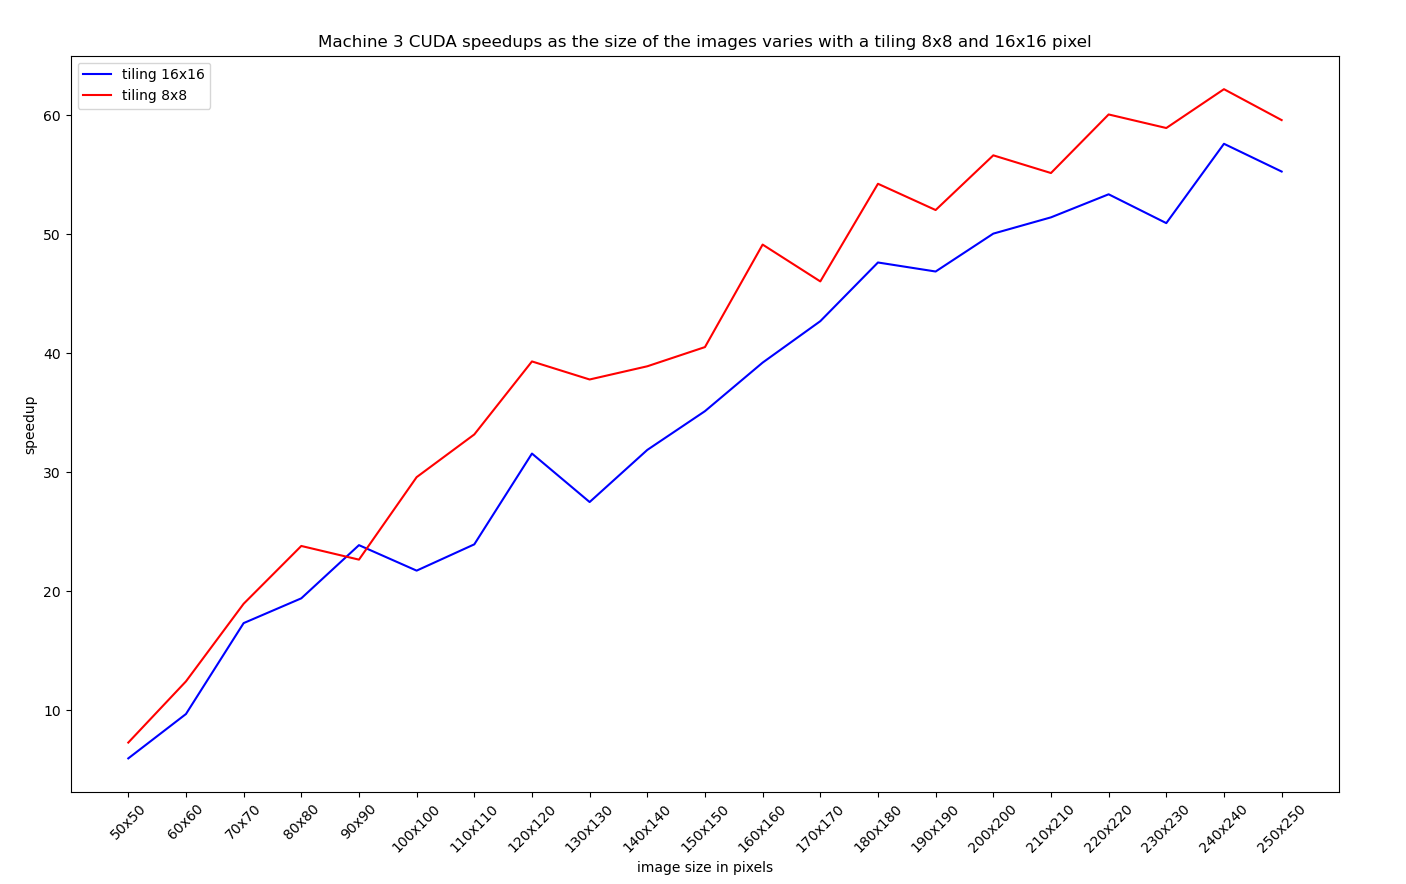
\includegraphics[width= 13cm]{"Immagini/Speedups_Varying_Size.PNG"}
\caption{Machine $ 3 $ CUDA speedups as the size of the images varies}
\label{Speedups_Varying_Size}
\end{figure}

\begin{figure}[!h]
\centering
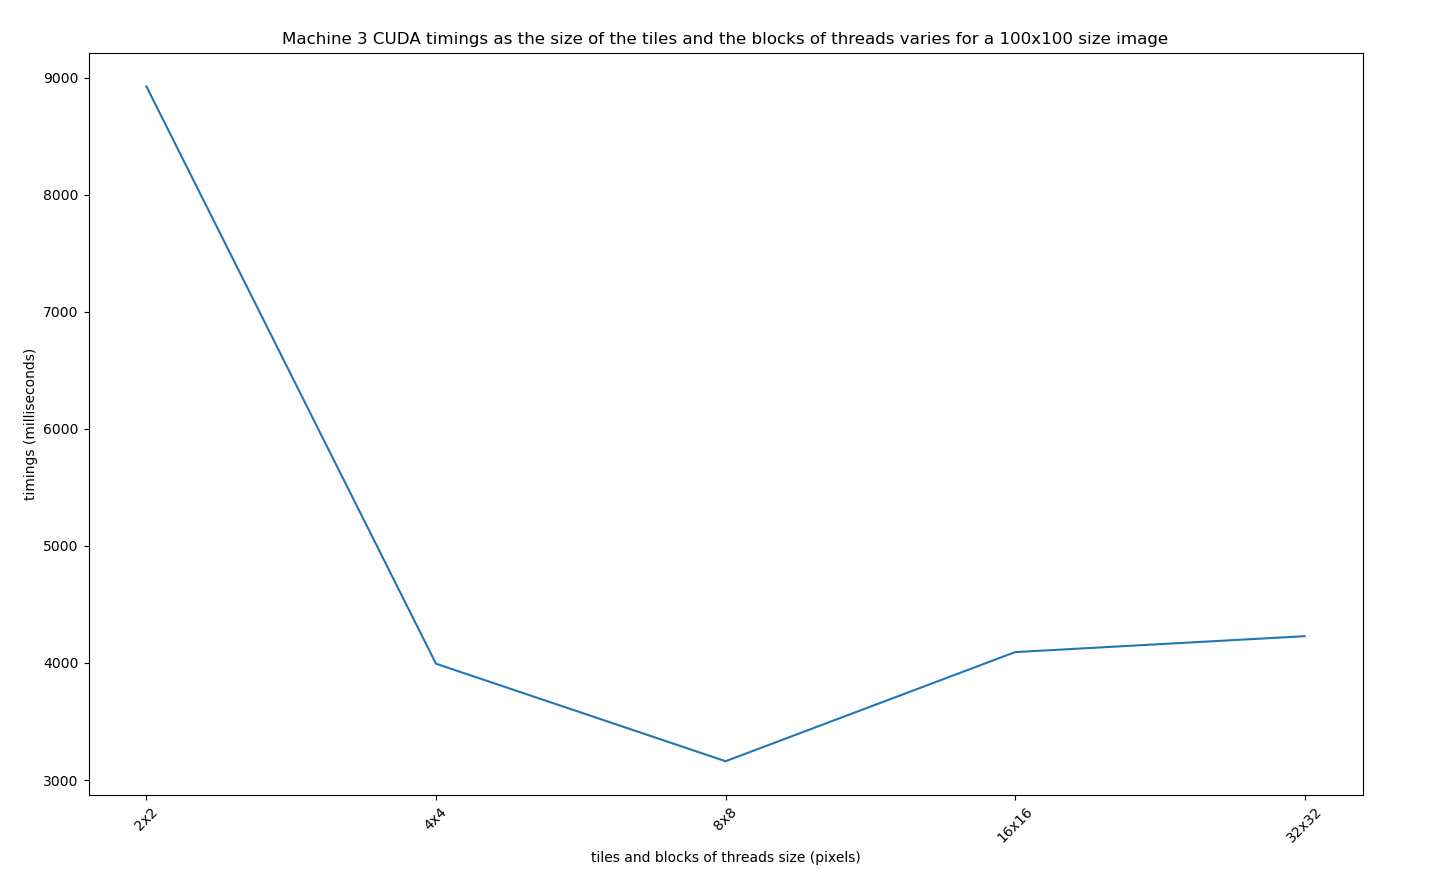
\includegraphics[width= 13cm]{"Immagini/Timings_Varying_Tiles.PNG"}
\caption{Machine $ 3 $ CUDA timings as the size of the tiles varies}
\label{Timings_Varying_Tile}
\end{figure}

\end{center}

\newpage

\section{Analisi e Conclusioni}

Come \'e possibile osservare in Tabella \ref{Timings} e \ref{Speedups}, la parallelizzazione tramite OpenMP della versione dell’algoritmo Mean Shift implementata con la struttura SoA risulta pi\'u vantaggiosa quando applicata alla macchina $ 1 $. Questo impatto \'e dovuto alla peculiarit\'a di quest’ultima di essere pi\'u facilmente allineabile con la memoria cache; tuttavia, come si può notare dai risultati ottenuti con la macchina $ 2 $, i vantaggi di questa struttura non sono sempre apprezzabili, poich\'e probabilmente sensibili all'architettura hardware.\\
Lo speedup ottenuto risulta comunque sublineare per entrambe le versioni, mostrandosi più o meno alto a seconda della potenza specifica di ogni singola macchina.\\
La parallelizzazione tramite CUDA in GPU risulta, come ipotizzabile, nettamente maggiore rispetto alla parallelizzazione con OpenMP sempre proporzionalmente alle specifiche tecniche delle singole macchine. In particolare la Macchina $ 3 $ raggiunge uno speedup che, come si pu\'o osservare nel grafico di figura \ref{Speedups_Varying_Size}, continua a crescere all'aumentare della dimensione dell'immagine da clusterizzare. Quest'ultimo aspetto dimostra come le architetture GPU siano pi\'u performanti pi\'u \'e alta la dimensione dei dati in ingresso, poich\'e riescono a sfruttare maggiormente l'elevato numero di unit\'a di computazione. Infine, come apprezzabile in figura \ref{Speedups_Varying_Size} e \ref{Timings_Varying_Tile}, la dimensione dei tile e del numero di thread per blocco utilizzati impatta sui tempi di esecuzione ottenendo un minimo per la dimensione $8\times8$.  

\end{document}